\section{Double Integration and Volume}\label{sec:double_int_volume}

The definite integral of $f$ over $[a,b]$, $\int_a^b f(x)\ dx$, was introduced as ``the signed area under the curve.'' We approximated the value of this area by first subdividing $[a,b]$ into $n$ subintervals, where the $i^\text{ th}$ subinterval has length $\Delta x_i$, and letting $c_i$ be any value in the $i^\text{ th}$ subinterval. We formed rectangles that approximated part of the region under the curve with width $\Delta x_i$, height $f(c_i)$, and hence with area $f(c_i)\Delta x_i$. Summing all the rectangle's areas gave an approximation of the definite integral, and \autoref{thm:riemannSum} stated that
\[\int_a^bf(x)\ dx = \lim_{\|\Delta x\|\to 0}\sum f(c_i)\Delta x_i,\]
connecting the area under the curve with sums of the areas of rectangles.\bigskip

We use a similar approach in this section to find volume under a surface.\bigskip

Let $R$ be a closed, bounded region in the $x$-$y$ plane and let $z=f(x,y)$ be a continuous function defined on $R$. We wish to find the signed volume under the surface of $f$ over $R$. (We use the term ``signed volume'' to denote that space above the $x$-$y$ plane, under $f$, will have a positive volume; space above $f$ and under the $x$-$y$ plane will have a ``negative'' volume, similar to the notion of signed area used before.)

\mtable{Developing a method for finding signed volume under a surface.}{fig:double_intro}{%
\begin{tikzpicture}
\begin{axis}[width=1.16\marginparwidth,tick label style={font=\scriptsize},
axis y line=middle,axis x line=middle,name=myplot,axis on top,
ymin=-.85,ymax=.85,xmin=-.3,xmax=2.2]
\addplot [smooth,very thick, draw={\colorone},samples=40,domain=-90:90]
 ({cos(x)*(1+cos(2*x))},{sin(x)*(1+cos(2*x))});
\foreach \x/\y in { 0/.3 , .2/.4 , .4/.6 , .6/.7 , .8/.8 , 1/.8 , 1.2/.8 , 1.4/.8 , 1.6/.7 , 1.8/.6 , 2/.4 } {
 \edef\temp{\noexpand\draw(axis cs:\x,-\y)--(axis cs:\x,\y);}\temp
}
\foreach \x/\y/\z in { .8/.8/1.4 , .6/.7/1.6 , .4/.6/1.8 , .4/.5/1.8 , .2/.4/2 , 0/.3/2 , 0/.2/2 , 0/.1/2 , 0/-.1/2 , 0/-.2/2 , 0/-.3/2 , .2/-.4/2 , .4/-.5/1.8 , .4/-.6/1.8 , .6/-.7/1.6 , .8/-.8/1.4 } {
 \edef\temp{\noexpand\draw(axis cs:\x,\y)--(axis cs:\z,\y);}\temp
}
\end{axis}
\node [right] at (myplot.right of origin) {\scriptsize $x$};
\node [above] at (myplot.above origin) {\scriptsize $y$};
\end{tikzpicture}
\\(a)\\
\myincludeasythree{width=\marginparwidth,
3Droll=0,
3Dortho=0.005025407765060663,
3Dc2c=0.6666666865348816 0.6666666865348816 0.3333333730697632,
3Dcoo=5.279583930969238 -29.517940521240234 48.47616195678711,
3Droo=150.0000012715658}{width=\marginparwidth}{figures/figdouble_intro2_3D}
\\(b)}

We start by partitioning $R$ into $n$ rectangular subregions as shown in \autoref{fig:double_intro}(a). For simplicity's sake, we let all widths be $\Delta x$ and all heights be $\Delta y$. Note that the sum of the areas of the rectangles is not equal to the area of $R$, but rather is a close approximation. Arbitrarily number the rectangles 1 through $n$, and pick a point $(x_i,y_i)$ in the $i^\text{ th}$ subregion. 

The volume of the rectangular solid whose base is the $i^\text{ th}$ subregion and whose height is $f(x_i,y_i)$ is $V_i=f(x_i,y_i)\Delta x\Delta y$. Such a  solid is shown in \autoref{fig:double_intro}(b). Note how this rectangular solid only approximates the true volume under the surface; part of the solid is above the surface and part is below.

For each subregion $R_i$ used to approximate $R$, create the rectangular solid with base area $\Delta x\Delta y$ and height $f(x_i,y_i)$. The sum of all rectangular solids is
\[\ds \sum_{i=1}^n f(x_i,y_i)\Delta x\Delta y.\]
This approximates the signed volume under $f$ over $R$. As we have done before, to get a better approximation we can use more rectangles to approximate the region $R$.

In general, each rectangle could have a different width $\Delta x_j$ and height $\Delta y_k$, giving the $i^\text{ th}$ rectangle an area $\Delta A_i = \Delta x_j\Delta y_k$ and the $i^\text{ th}$ rectangular solid a volume of $f(x_i,y_i)\Delta A_i$. Let $\norm{\Delta A}$ denote the length of the longest diagonal of all rectangles in the subdivision of $R$; $\norm{\Delta A}\to 0$ means each rectangle's width and height are both approaching 0. If $f$ is a continuous function, as $\norm{\Delta A}$ shrinks (and hence $n\to\infty$) the summation $\ds \sum_{i=1}^n f(x_i,y_i)\Delta A_i$ approximates the signed volume better and better. This leads to a definition.

\mnote{\textbf{Note:} Recall that the integration symbol ``$\int$'' is an ``elongated S,'' representing the word ``sum.'' We interpreted $\int_a^bf(x)\ dx$ as ``take the \emph{sum} of the areas of rectangles over the interval $[a,b]$.'' The double integral uses two integration symbols to represent a ``double sum.'' When adding up the volumes of rectangular solids over a partition of a region $R$, as done in \autoref{fig:double_intro}, one could first add up the volumes across each row (one type of sum), then add these totals together (another sum), as in
\[\sum_{j=1}^n\sum_{i=1}^mf(x_i,y_j)\Delta x_i\Delta y_j.\]
One can rewrite this  as
\[\sum_{j=1}^n\left(\sum_{i=1}^mf(x_i,y_j)\Delta x_i\right)\Delta y_j.\]
The summation inside the parenthesis indicates the sum of  heights $\times$ widths, which gives an area; multiplying these areas by the thickness $\Delta y_j$ gives a volume. The illustration in \autoref{fig:double_intro3} relates to this understanding.\label{note:doubleint}}

\begin{definition}[Double Integral, Signed Volume]\label{def:double_int}
Let $z=f(x,y)$ be a continuous function defined over a closed region $R$ in the $x$-$y$ plane. The \textbf{signed volume} $V$ under $f$ over $R$ is denoted by the \textbf{double integral}\vspace{-.5\baselineskip}
\[V = \iint_R f(x,y)\ dA.\]
Alternate notations for the double integral are
\index{integration!double}\index{double integral}\index{iterated integration}\index{signed volume}\index{volume}
\[\iint_R f(x,y)\ dA=\iint_R f(x,y)\ dx\ dy=\iint_R f(x,y)\ dy\ dx.\]
\end{definition}

The definition above does not state how to find the signed volume, though the notation offers a hint. We need the next two theorems to evaluate double integrals to find volume.

\begin{theorem}[Double Integrals and Signed Volume]\label{thm:double_int}
Let $z=f(x,y)$ be a continuous function defined over a closed region $R$ in the $x$-$y$ plane. Then the signed volume $V$ under $f$ over $R$ is
\[V = \iint_R f(x,y)\ dA = \lim_{\norm{\Delta A}\to 0}\sum_{i=1}^n f(x_i,y_i)\Delta A_i.\]
\end{theorem}

This theorem states that we can find the exact signed volume using a limit of sums. The partition of the region $R$ is not specified, so any partitioning where the diagonal of each rectangle shrinks to 0 results in the same answer. 

This does not offer a very satisfying way of computing volume, though. Our experience has shown that evaluating the limits of sums can be tedious. We seek a more direct method.

Recall \autoref{thm:volume_by_cross_section} in \autoref{sec:disk}. This stated that if $A(x)$ gives the cross-sectional area of a solid at $x$, then $\int_a^b A(x)\ dx$ gave the volume of that solid over $[a,b]$. 

Consider \autoref{fig:double_intro3}, where a surface $z=f(x,y)$ is drawn over a region $R$. Fixing a particular $x$ value, we can consider the area under $f$ over $R$ where $x$ has that fixed value. That area can be found with a definite integral, namely
\[ A(x)=\int_{g_1(x)}^{g_2(x)} f(x,y)\ dy.\]

Remember that though the integrand contains $x$, we are viewing $x$ as fixed. Also note that the bounds of integration are functions of $x$: the bounds depend on the value of $x$. 

\mtable{Finding volume under a surface by sweeping out a cross-sectional area.}{fig:double_intro3}{%
\myincludeasythree{width=\marginparwidth,
3Droll=0,
3Dortho=0.005067072808742523,
3Dc2c=0.5451613068580627 0.7846456170082092 0.29517868161201477,
3Dcoo=9.929030418395996 -41.68748092651367 56.98992919921875,
3Droo=200.99999858350685}{width=\marginparwidth}{figures/figdouble_intro3_3D}}

As $A(x)$ is a cross-sectional area function, we can find the signed volume $V$ under $f$ by integrating it:
\[
V = \int_a^b A(x)\ dx = \int_a^b\left(\int_{g_1(x)}^{g_2(x)} f(x,y)\ dy\right)dx
= \int_a^b\int_{g_1(x)}^{g_2(x)} f(x,y)\ dy\ dx.
\]

This gives a concrete method for finding signed volume under a surface. We could do a similar procedure where we started with $y$ fixed, resulting in a iterated integral with the order of integration $dx\ dy$. The following theorem states that both methods give the same result, which is the value of the double integral. It is such an important theorem it has a name associated with it.

\begin{theorem}[Fubini's Theorem]\label{thm:fubini}
Let $R$ be a closed, bounded region in the $x$-$y$ plane and let $z=f(x,y)$ be a continuous function on $R$.%
\index{double integral}\index{iterated integration}\index{signed volume}\index{volume}\index{Fubini's Theorem}
\begin{enumerate}
	\item If $R$ is bounded by $a\leq x\leq b$ and $g_1(x)\leq y\leq g_2(x)$, where $g_1$ and $g_2$ are continuous functions on $[a,b]$, then
	\[\iint_R f(x,y)\ dA = \int_a^b\int_{g_1(x)}^{g_2(x)} f(x,y)\ dy\ dx.\]
	
	\item If $R$ is bounded by $c\leq y\leq d$ and $h_1(y)\leq x\leq h_2(y)$, where $h_1$ and $h_2$ are continuous functions on $[c,d]$, then
	\[\iint_R f(x,y)\ dA = \int_c^d\int_{h_1(y)}^{h_2(y)} f(x,y)\ dx\ dy.\]
\end{enumerate}
\end{theorem}

Note that the bounds of integration follow a ``curve to curve, point to point'' pattern. In fact, one of the main points of the previous section is developing the skill of describing a region $R$ with the bounds of an iterated integral. Once this skill is developed, we can use double integrals to compute many quantities, not just signed volume under a surface.

\youtubeVideo{NG2UcXdwzfk}{Ex: Evaluate a Double Integral to Determine Volume (Basic)}

\begin{example}[Evaluating a double integral]\label{ex_double1}
Let $f(x,y) = xy+e^y$. Find the signed volume under $f$ on the region $R$, which is the rectangle with corners $(3,1)$ and $(4,2)$ pictured in \autoref{fig:double1}, using Fubini's Theorem and both orders of integration.
\solution
We wish to evaluate $\iint_R \bigl(xy+e^y\bigr)\ dA$. As $R$ is a rectangle, the bounds are easily described as $3\leq x\leq 4$ and $1\leq y\leq 2$.\bigskip

\mtable{Finding the signed volume under a surface in \autoref{ex_double1}.}{fig:double1}{%
\myincludeasythree{width=\marginparwidth,
3Droll=0.,
3Dortho=0.0046491301618516445,
3Dc2c=0.5071550607681274 -0.7884454131126404 0.3480626046657562,
3Dcoo=34.443328857421875 108.33967590332031 55.163639068603516,
3Droo=149.99999646067835}{width=\marginparwidth}{figures/figdouble1_3D}}

Using the order $dy\ dx$:
\begin{align*}
\iint_R\bigl(xy+e^y\bigr) \ dA
	&= \int_3^4\int_1^2\bigl(xy+e^y\bigr)\ dy \ dx \\
	&= \int_3^4 \left(\left.\left[\frac12xy^2+e^y\right]\right|_1^2\ \right) dx \\
	&= \int_3^4\left(\frac 32x + e^2-e\right)dx \\
	&= \left.\left(\frac 34x^2 + \bigl(e^2-e\bigr)x\right)\right|_3^4 \\
	&= \frac {21}4+ e^2-e%\approx 9.92
	.
\end{align*}

Now we check the validity of Fubini's Theorem by using the order $dx\ dy$:
\allowdisplaybreaks
\begin{align*}
\iint_R\bigl(xy+e^y\bigr) \ dA &= \int_1^2\int_3^4\bigl(xy+e^y\bigr)\ dx \ dy \\
		&= \int_1^2\left(\left.\left[\frac12x^2y+xe^y\right]\right|_3^4\right)dy\\
		&= \int_1^2\left(\frac72y+e^y\right)\ dy\\
		&= \left.\left(\frac74y^2+e^y\right)\right|_1^2\\
		&=\frac{21}4+e^2-e%\approx 9.92
		.
\end{align*}
Both orders of integration return the same result, as expected.
\end{example}

%\begin{example}[Evaluating a double integral]\label{ex_double2}
%Evaluate $\iint_R e^{2x+3y}\ dA$, where $R$ is the triangle bounded by $x=0$, $y=0$ and $\frac12x+y=1$, as shown in FIGURE.
%\solution
%While it is not specified which order we are to use, we will evaluate the double integral using both orders to help drive home the point that it does not matter which order we use.\\
%
%Using the order $dy\ dx$:
%The bounds on $y$ go from ``curve to curve,'' i.e., $0\leq y\leq 1-x/2$, and the bounds on $x$ go from ``point to point,'' i.e., $0\leq x\leq 2$.
%\begin{align*}
%\iint_R e^{2x+3y}\ dA &= \int_0^2\int_0^{-\frac x2+1} e^{2x+3y}\ dy\ dx\\
		%&= \int_0^2\left.\left(\frac13e^{2x+3y}\right)\right|_0^{-\frac x2+1}dx\\
		%&= \int_0^2 \left(\frac13\left(e^{\frac x2+3}-e^{2x}\right)\right)dx \\
		%&= \frac13\left.\left(2e^{\frac x2+3}-\frac12e^{2x}\right)\right|_0^2\\
		%&= \frac13\left(\frac32e^4-2e^3+\frac12\right)\\
		%&= \frac12e^4-\frac23e^3+\frac16%\approx  14.08
		%.
%\end{align*}
%
%Now lets consider the order $dx \ dy$. Here $x$ goes from ``curve to curve,'' $0\leq x\leq 2-2y$, and $y$ goes from ``point to point,'' $0\leq y\leq 1$:
%\begin{align*}
%\iint_R e^{2x+3y}\ dA &= \int_0^1\int_0^{2-2y} e^{2x+3y}\ dy\ dx\\
		%&= \int_0^1\left.\left(\frac12e^{2x+3y}\right)\right|_0^{2-2y} dy\\
		%&= \int_0^1\left(\frac12\bigl(e^{4-y}-e^{3y}\bigr)\right)dy\\
		%&=\left.\frac12\left(-e^{4-y}-\frac13e^{3y}\right)\right|_0^1\\
		%&=\frac12\left(-\frac43e^3+e^4+\frac13\right)\\
		%&= \frac12e^4-\frac23e^3+\frac16%\approx  14.08
		%.
%\end{align*}
%We obtained the same result using both orders of integration.
%\end{example}

\begin{example}[Evaluating a double integral]\label{ex_double2}
Evaluate $\iint_R \bigl(3xy-x^2-y^2+6\bigr)\ dA$, where $R$ is the triangle bounded by $x=0$, $y=0$ and $x/2+y=1$, as shown in \autoref{fig:double2}.
\solution
While it is not specified which order we are to use, we will evaluate the double integral using both orders to help drive home the point that it does not matter which order we use.

\mtable{Finding the signed volume under the surface in \autoref{ex_double2}.}{fig:double2}{%
\myincludeasythree{width=\marginparwidth,
3Droll=0,
3Dortho=0.0046491301618516445,
3Dc2c=0.3019719421863556 -0.9206370115280151 0.24746793508529663,
3Dcoo=45.67414093017578 112.43929290771484 56.7108039855957,
3Droo=200.99999432688844}{width=\marginparwidth}{figures/figdouble2_3D}}

Using the order $dy\ dx$:
The bounds on $y$ go from ``curve to curve,'' i.e., $0\leq y\leq 1-x/2$, and the bounds on $x$ go from ``point to point,'' i.e., $0\leq x\leq 2$.
\begin{align*}
\iint_R (3xy-x^2-y^2+6\bigl)\ dA &= \int_0^2\int_0^{-\frac x2+1} (3xy-x^2-y^2+6\bigr)\ dy\ dx\\
		&= \int_0^2\left.\left(\frac32xy^2-x^2y-\frac13y^3+6y\right)\right|_0^{-\frac x2+1}dx\\
		&= \int_0^2 \left(\frac{11}{12}x^3-\frac{11}{4}x^2-x+\frac{17}3\right)dx \\
		&= \left.\left(\frac{11}{48}x^4-\frac{11}{12}x^3-\frac12x^2+\frac{17}3x\right)\right|_0^2\\
		&= \frac{17}3=5.\overline{6}.
\end{align*}

Now lets consider the order $dx \ dy$. Here $x$ goes from ``curve to curve,'' $0\leq x\leq 2-2y$, and $y$ goes from ``point to point,'' $0\leq y\leq 1$:
{\allowdisplaybreaks
\begin{align*}
\iint_R \bigl(3xy-x^2-y^2+6\bigr)\ dA
	&= \int_0^1\int_0^{2-2y} \bigl(3xy-x^2-y^2+6\bigr)\ dx\ dy\\
	&= \int_0^1\left.\left(\frac32x^2y-\frac13x^3-xy^2+6x\right)\right|_0^{2-2y} dy\\
	&= \int_0^1\left(\frac{32}3y^3-22y^2+2y+\frac{28}3\right)dy\\
	&=\left.\left(\frac83y^4-\frac{22}3y^3+y^2+\frac{28}3y\right)\right|_0^1\\
	&=\frac{17}3=5.\overline{6}.
\end{align*}}
We obtained the same result using both orders of integration.
\end{example}

Note how in these two examples that the bounds of integration depend only on $R$; the bounds of integration have nothing to do with $f(x,y)$. This is an important concept, so we include it  as a Key Idea.

\begin{keyidea}[Double Integration Bounds]\label{idea:bounds_on_double}
When evaluating $\iint_Rf(x,y)\ dA$ using an iterated integral, the bounds of integration depend only on $R$. The surface $f$ does not determine the bounds of integration.
\end{keyidea}

Before doing another example, we give some properties of double integrals. Each should make sense if we view them in the context of finding signed volume under a surface, over a region.

\begin{theorem}[Properties of Double Integrals]\label{thm:double_prop}
Let $f$ and $g$ be continuous functions over a closed, bounded plane region $R$, and let $c$ be a constant.
\index{double integral!properties}\index{iterated integration!properties}
\begin{enumerate}
	\item $\ds \iint_Rc\,f(x,y)\ dA = c\iint_Rf(x,y)\ dA.$
	\item	$\ds \iint_R \bigl(f(x,y)\pm g(x,y)\bigr)\ dA = \iint_R f(x,y)\ dA \pm \iint_R g(x,y)\ dA $
	\item	If $f(x,y)\geq 0$ on $R$, then $\ds \iint_R f(x,y)\ dA\geq 0$.
	\item	If $f(x,y)\geq g(x,y)$ on $R$, then $\ds \iint_R f(x,y)\ dA\geq \iint_R g(x,y)\ dA$.
%
% todo parameterize this instead of a bunch of coordinates
\mtable[-2in]{$R$ is the union of two nonoverlapping regions, $R_1$ and $R_2$.}{fig:double_region}{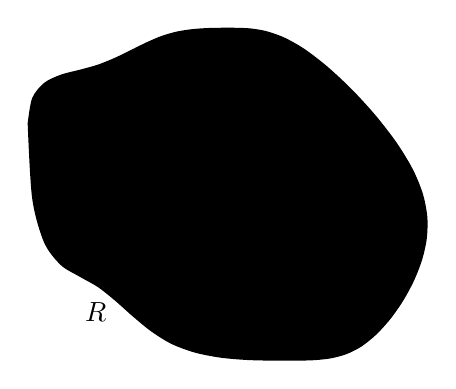
\begin{tikzpicture}[xscale=.85,yscale=.6]
\draw [draw={\colorone},thick,fill={\coloronefill},smooth] plot coordinates {(0,2.)
(0.06639,2.527)(0.2407,2.839)(0.4857,3.009)(0.7641,3.112)(1.039,3.221)(1.294,3.367)
(1.532,3.53)(1.759,3.689)(1.98,3.823)(2.2,3.915)(2.42,3.967)(2.64,3.992)(2.86,4.)
(3.08,4.)(3.305,3.987)(3.543,3.93)(3.808,3.797)(4.107,3.558)(4.45,3.185)(4.815,2.703)
(5.17,2.152)(5.483,1.577)(5.723,1.018)(5.872,0.5022)(5.938,0.02083)(5.93,-0.4363)
(5.861,-0.88)(5.741,-1.319)(5.58,-1.742)(5.389,-2.128)(5.179,-2.456)(4.96,-2.705)
(4.737,-2.865)(4.502,-2.953)(4.243,-2.991)(3.95,-3.)(3.614,-2.999)(3.244,-2.984)
(2.86,-2.935)(2.484,-2.829)(2.137,-2.646)(1.832,-2.378)(1.558,-2.06)(1.299,-1.734)
(1.039,-1.443)(0.7641,-1.222)(0.4857,-0.9779)(0.2407,-0.5015)(0.06639,0.4201)(0,2.)};
\draw [thick,draw={\colorone}] (3,4) -- (4,-3);
\draw (2,1) node {$R_1$};
\draw (5,.5) node {$R_2$};
\draw (1,-2) node {$R$};
\end{tikzpicture}}
%
	\item \label{thm:double_prop_regions}	Let $R$ be the union of two nonoverlapping regions, $R = R_1\bigcup R_2$ (see \autoref{fig:double_region}). Then 
	\[\iint_R f(x,y)\ dA = \iint_{R_1}f(x,y)\ dA+ \iint_{R_2}f(x,y)\ dA.\]
\end{enumerate}
\end{theorem}

\begin{example}[Evaluating a double integral]\label{ex_double3}
Let $f(x,y) = \sin x\cos y$ and $R$ be the triangle with vertices $(-1,0)$, $(1,0)$ and $(0,1)$ (see \autoref{fig:double3}). Evaluate the double integral $\iint_Rf(x,y)\ dA$.
%
\mtable{Finding the signed volume under a surface in \autoref{ex_double3}.}{fig:double3}{%
\myincludeasythree{width=\marginparwidth,
3Droll=0.,
3Dortho=0.0046491301618516445,
3Dc2c=0.08563969284296036 0.8920179605484009 0.44381290674209595,
3Dcoo=-0.3899505138397217 30.125946044921875 17.537517547607422,
3Droo=200.9999927619444}{width=\marginparwidth}{figures/figdouble3_3D}}
\solution
If we attempt to integrate using an iterated integral with the order $dy\ dx$, note how there are two upper bounds on $R$ meaning we'll need to use two iterated integrals. We would need to split the triangle into two regions along the $y$-axis, then use \autoref{thm:double_prop}, part \ref{thm:double_prop_regions}.

Instead, let's use the order $dx\ dy$. The curves bounding $x$ are $y-1\leq x\leq 1-y$; the bounds on $y$ are $0\leq y\leq 1$. This gives us:
\begin{align*}
\iint_R f(x,y)\ dA &= \int_0^1\int_{y-1}^{1-y}\sin x\cos y\ dx\ dy\\
		&= \int_0^1\left.\Bigl( -\cos x\cos y\Bigr)\right|_{y-1}^{1-y}dy\\
		&= \int_0^1 \cos y\Bigl(-\cos (1-y) + \cos(y-1)\Bigr)dy.
\end{align*}
Recall that the cosine function is an even function; that is, $\cos x = \cos (-x)$. Therefore, from the last integral above, we have $\cos (y-1) = \cos (1-y)$. Thus the integrand simplifies to 0, and we have 
\begin{align*}
\iint_R f(x,y)\ dA &= \int_0^1 0\ dy \\
&= 0.
\end{align*}
It turns out that over $R$, there is just as much volume above the $x$-$y$ plane as below (look again at \autoref{fig:double3}), giving a final signed volume of 0.
\end{example}

\begin{example}[Evaluating a double integral]\label{ex_double4}
Evaluate $\iint_R (4-y)\ dA$, where $R$ is the region bounded by the parabolas $y^2=4x$ and $x^2=4y$, graphed in \autoref{fig:double4}.
%
\mtable{Finding the volume under the surface in \autoref{ex_double4}.}{fig:double4}{%
\myincludeasythree{width=\marginparwidth,
3Droll=0,
3Dortho=0.004656145814806223,
3Dc2c=0.9017289280891418 0.24087461829185486 0.35897672176361084,
3Dcoo=-13.985211372375488 45.56017303466797 41.332950592041016,
3Droo=201.0000081559461}{width=\marginparwidth}{figures/figdouble4_3D}}
%
\solution
Graphing each curve can help us find their points of intersection. Solving analytically, the second equation tells us that $y=x^2/4$. Substituting this value in for $y$ in the first equation gives us $x^4/16 = 4x$. Solving for $x$:
\begin{align*}
\frac{x^4}{16} &= 4x\\
x^4-64x &=0\\
x(x^3-64) &=0\\
x&= 0,\ 4.
\end{align*}
Thus we've found analytically what was easy to approximate graphically: the regions intersect at $(0,0)$ and $(4,4)$, as shown in \autoref{fig:double4}. 

We now choose an order of integration: $dy\ dx$ or $dx\ dy$? Either order works; since the integrand does not contain $x$, choosing $dx\ dy$ might be simpler --- at least, the first integral is very simple.

Thus we have the following ``curve to curve, point to point'' bounds: $y^2/4\leq x\leq 2\sqrt y$, and $0\leq y\leq 4$. 
\begin{align*}
\iint_R &(4-y)\ dA \\
	&= \int_0^4\int_{y^2/4}^{2\sqrt{y}}(4-y)\ dx\ dy\\
	&= \int_0^4 \bigl(x(4-y)\bigr)\Big|_{y^2/4}^{2\sqrt{y}} dy\\
	&= \int_0^4 \Bigl(\bigl(2\sqrt{y}-\frac{y^2}{4}\bigr)\bigl(4-y\bigr)\Bigr)\ dy = \int_0^4 \Bigl( \frac{y^3}{4}-y^2-2y^{3/2}+8y^{1/2}\Bigr)\ dy\\
	&= \left.\left(\frac{y^4}{16}-\frac{y^3}{3}-\frac{4y^{5/2}}5+\frac{16y^{3/2}}3\right)\right|_0^4\\
	&= \frac{176}{15} = 11.7\overline{3}.
\end{align*}
The signed volume under the surface $f$ is about 11.7 cubic units.
\end{example}

%\subsection{Changing Order of Integration}
%
%In each of the previous examples, we have been given a region to integrate over and found the bounds needed for the order of integration chosen. Sometimes, to establish their equality, we integrated with both orders of operation.
%
%We now approach the skill of describing a region using both orders of integration from a different perspective. Instead of starting with a region and creating iterated integrals, we will start with an iterated integral and rewrite it in the other integration order. To do so, we'll need to understand the region over which we are integrating.
%
%The simplest of all cases is when both integrals are bound by constants. The region described by these bounds is a rectangle (see \autoref{ex_double1}), and so:
%\[\int_a^b\int_c^d f(x,y)\ dy\ dx = \int_c^d\int_a^bf(x,y)\ dx\ dy.\]
%
%When the inner integral's bounds are not constants, it is generally very useful to sketch the bounds to determine what the region we are integrating over looks like. From the sketch we can then rewrite the integral with the other order of integration.
%
%Examples will help us develop this skill.
%
%\begin{example}[Changing the order of integration]\label{ex_double5}
%Rewrite the iterated integral $\ds \int_0^6\int_0^{x/3} \frac{x}{x^2+y^2+1}\ dy\ dx$ with the order of integration $dx\ dy$.
%\solution
%We need to use the bounds of integration to determine the region we are integrating over. Recall \autoref{idea:bounds_on_double}: the region $R$ is completely determined by these bounds, and not influenced at all by the integrand. Therefore, to rewrite the integral, we ignore the integrand.
%
%The bounds tell us that $y$ is bounded by $0$ and $x/3$; $x$ is bounded by 0 and 6. We plot these four curves: $y=0$, $y=x/3$, $x=0$ and $x=6$ to find the region described by the bounds. \autoref{fig:double5} shows these curves, indicating that $R$ is a triangle.
%\mtable{Sketching the region $R$ described by the iterated integral in \autoref{ex_double5}.}{fig:double5}{\begin{tikzpicture}
%\begin{axis}[width=1.16\marginparwidth,tick label style={font=\scriptsize},
%axis y line=middle,axis x line=middle,name=myplot,axis on top,
%ymin=-.5,ymax=2.5,xmin=-.5,xmax=6.9]
%\draw [very thick,draw={\colortwo}] (axis cs:-.5,0) -- (axis cs:6.9,0)
%	(axis cs:-.5,-.1666)
%	-- node [above,black,pos=.5,sloped] {\scriptsize $y=x/3$} (axis cs: 6.9, 2.3);
%\draw [very thick,draw={\colorone}] (axis cs:0,-.5) -- (axis cs:0,2.5)
%	(axis cs:6,-.5) -- (axis cs:6,2.5);
%\draw (axis cs:4,.5) node {$R$};													
%\end{axis}
%\node [right] at (myplot.right of origin) {\scriptsize $x$};
%\node [above] at (myplot.above origin) {\scriptsize $y$};
%\end{tikzpicture}}
%
%To change the order of integration, we need to consider the curves that bound the $x$-values. We see that the lower bound is $x=3y$ and the upper bound is $x=6$. The bounds on $y$ are $0$ to $2$. Thus we can rewrite the integral as 
%$\ds \int_0^2\int_{3y}^6 \frac{x}{x^2+y^2+1}\ dx \ dy.$
%\end{example}
%
%\begin{example}[Changing the order of integration]\label{ex_double7}
%Change the order of integration of $\ds\int_0^2\int_{y^2/4}^{(y+4)/2}f(x,y)\ dx\ dy$.
%\solution
%We sketch the region described by the bounds to help us change the integration order. We see $x$ is bounded below and above (i.e., to the left and right) by $x=y^2/4$ and $x=(y+4)/2$ respectively, and $y$ is bounded between 0 and 2. Graphing the previous curves, we find the region $R$ to be that shown in \autoref{fig:double7}. 
%\mtable{Drawing the region determined by the bounds of integration in \autoref{ex_double7}.}{fig:double7}{\begin{tikzpicture}
%\begin{axis}[width=1.16\marginparwidth,tick label style={font=\scriptsize},
%axis y line=middle,axis x line=middle,name=myplot,axis on top,
%ymin=-.5,ymax=4.5,xmin=-.5,xmax=4.5]
%\addplot [smooth,very thick,draw={\colorone},samples=10,domain=-.5:4.5] ({x^2/4},{x});
%\addplot [smooth,very thick,draw={\colorone},samples=10,domain=-.5:4.5] ({((x+4))/2},{x});
%\draw [very thick,draw={\colortwo}] (axis cs:-.5,0) -- (axis cs:4.5,0)
%	(axis cs:-.5,4) -- (axis cs:4.5,4);
%\draw (axis cs:2,1.75) node {$R$};													
%\draw (axis cs:2,3.1) node [rotate=30] {\scriptsize$x=y^2/4$};
%\draw (axis cs:3,1.5) node [rotate=56] {\scriptsize $x= (y+4)/2$};
%\end{axis}
%\node [right] at (myplot.right of origin) {\scriptsize $x$};
%\node [above] at (myplot.above origin) {\scriptsize $y$};
%\end{tikzpicture}}
%
%To change the order of integration, we need to establish curves that bound $y$. The figure makes it clear that there are two lower bounds for $y$: $y=0$ on $0\leq x\leq 2$, and $y=2x-4$ on $2\leq x\leq 4$. Thus we need two double integrals. The upper bound for each is $y=2\sqrt{x}$. Thus we have
%\[\int_0^2\int_{y^2/4}^{(y+4)/2}f(x,y)\ dx\ dy = \int_0^2\int_0^{2\sqrt{x}} f(x,y)\ dy\ dx + \int_2^4\int_{2x-4}^{2\sqrt{x}}f(x,y)\ dy\ dx.\]
%Note how we did not specify the integrand, leaving it to be some function $f(x,y)$. This again stresses the point that the integrand has no bearing on the bounds of integration.
%\end{example}

In the previous section we practiced changing the order of integration of a given iterated integral, where the region $R$ was not explicitly given. Changing the bounds of an integral is more than just an test of understanding. Rather, there are cases where integrating in one order is really hard, if not impossible, whereas integrating with the other order is feasible.

\begin{example}[Changing the order of integration]\label{ex_double6}
Rewrite the iterated integral $\ds \int_0^3\int_y^3 e^{-x^2}\ dx\ dy$ with the order $dy\ dx$. Comment on the feasibility to evaluate each integral.
\solution
Once again we make a sketch of the region over which we are integrating to facilitate changing the order. The bounds on $x$ are from $x=y$ to $x=3$; the bounds on $y$ are from $y=0$ to $y=3$. These curves are sketched in \autoref{fig:double6}, enclosing the region $R$.

\mtable{Determining the region $R$ determined by the bounds of integration in \autoref{ex_double6}.}{fig:double6}{\begin{tikzpicture}
\begin{axis}[width=1.16\marginparwidth,tick label style={font=\scriptsize},
axis y line=middle,axis x line=middle,name=myplot,axis on top,
ymin=-.5,ymax=3.5,xmin=-.5,xmax=3.5]
\draw [very thick,draw={\colortwo}] (axis cs:-.5,0) -- (axis cs:3.5,0)
 (axis cs:-.5,3) -- (axis cs:3.5,3);
\draw [very thick,draw={\colorone}] (axis cs:3,-.5) -- (axis cs:3,3.5)
 (axis cs:-.5,-.5)
 -- node [above,black,pos=.5,sloped] {\scriptsize $y=x$} (axis cs: 3.5,3.5);
\draw (axis cs:2,1) node {$R$};                                                                                                 
\end{axis}
\node [right] at (myplot.right of origin) {\scriptsize $x$};
\node [above] at (myplot.above origin) {\scriptsize $y$};
\end{tikzpicture}}

To change the bounds, note that the curves bounding $y$ are $y=0$ up to $y=x$; the triangle is enclosed between $x=0$ and $x=3$. Thus the new bounds of integration are $0\leq y\leq x$ and $0\leq x\leq 3$, giving the iterated integral $\ds \int_0^3\int_0^x e^{-x^2}\ dy\ dx$.

How easy is it to evaluate each iterated integral? Consider the order of integrating $dx\ dy$, as given in the original problem. The first indefinite integral we need to evaluate is $\int e^{-x^2}\ dx$; we have stated before (see \autoref{sec:numerical_integration}) that this integral cannot be evaluated in terms of elementary functions. We are stuck.

Changing the order of integration makes a big difference here. In the second iterated integral, we are faced with $\int e^{-x^2}\ dy$; integrating with respect to $y$ gives us $ye^{-x^2}+C$, and the first definite integral evaluates to 
\[\int_0^x e^{-x^2}\ dy = xe^{-x^2}.\]
%
\mtable{Showing the surface $f$ defined in \autoref{ex_double6} over its region $R$.}{fig:double6b}{%
\myincludeasythree{width=\marginparwidth,
3Droll=0.,
3Dortho=0.005074724089354277,
3Dc2c=0.3949831426143646 0.8441238403320312 0.3625510632991791,
3Dcoo=41.500732421875 17.729557037353516 46.038082122802734,
3Droo=201.00002888349545}{width=\marginparwidth}{figures/figdouble6b_3D}}%
%
Thus 
\[
 \int_0^3\int_0^x e^{-x^2}\ dy\ dx
 = \int_0^3\Bigl(xe^{-x^2}\Bigr)dx
 = \int_0^9\frac12 e^{-u}\ du,
\]
where we used the substitution $u=x^2$, giving a final answer of $\frac12(1-e^{-9})%\approx 0.5
$. \autoref{fig:double6b} shows the surface over $R$.

In short, evaluating one iterated integral is impossible; the other iterated integral is relatively simple.
\end{example}

\autoref{def:av_val} defines the average value of a single-variable function $f(x)$ on the interval $[a,b]$ as
\[\text{average value of $f(x)$ on $[a,b]$} = \frac1{b-a}\int_a^b f(x)\ dx;\]
that is, it is the ``area under $f$ over an interval divided by the length of the interval.'' We make an analogous statement here: the average value of $z=f(x,y)$ over a region $R$ is the volume under $f$ over $R$ divided by the area of $R$.

\begin{definition}[The Average Value of $f$ on $R$]\label{def:av_val2}
Let $z=f(x,y)$ be a continuous function defined over a closed region $R$ in the $x$-$y$ plane. The \textbf{average value of $f$ on $R$} is \index{average value of a function}
\[\text{average value of $f$ on $R$} = \frac{\ds \iint_R f(x,y)\ dA}{\ds\iint_R \ dA}.\]
\end{definition}

\begin{example}[Finding average value of a function over a region $R$]\label{ex_double8}
Find the average value of $f(x,y) = 4-y$ over the region $R$, which is bounded by the parabolas $y^2=4x$ and $x^2=4y$. Note: this is the same function and region as used in \autoref{ex_double4}.
\solution
In \autoref{ex_double4} we found 
\[\iint_R f(x,y)\ dA = \int_0^4\int_{y^2/4}^{2\sqrt{y}}(4-y)\ dx\ dy = \frac{176}{15}.\] 
We find the area of $R$ by computing $\iint_R \ dA$:
\[\iint_R \ dA = \int_0^4\int_{y^2/4}^{2\sqrt{y}} \ dx\ dy = \frac{16}{3}.\]
%
\mtable{Finding the average value of $f$ in \autoref{ex_double8}.}{fig:double8}{%
\myincludeasythree{width=\marginparwidth,
3Droll=0,
3Dortho=0.004656145814806223,
3Dc2c=0.9017289280891418 0.24087461829185486 0.35897672176361084,
3Dcoo=-13.985211372375488 45.56017303466797 41.332950592041016,
3Droo=201.0000081559461}{width=\marginparwidth}{figures/figdouble4_3D}}%
%
Dividing the volume under the surface by the area gives the average value:
\[\text{average value of $f$ on $R$} = \frac{176/15}{16/3} = \frac{11}5 = 2.2.\]
While the surface, as shown in \autoref{fig:double8}, covers $z$-values from $z=0$ to $z=4$, the ``average'' $z$-value on $R$ is 2.2.
\end{example}

The previous section introduced the iterated integral in the context of finding the area of plane regions. This section has extended our understanding of iterated integrals; now we see they can be used to find the signed volume under a surface. 

This new understanding allows us to revisit what we did in the previous section. Given a region $R$ in the plane, we computed $\iint_R 1\ dA$; again, our understanding at the time was that we were finding the area of $R$. However, we can now view the function $z=1$ as a surface, a flat surface with constant $z$-value of 1. The double integral $\iint_R 1\ dA$ finds the volume, under $z=1$, over $R$, as shown in \autoref{fig:double_summary}. Basic geometry tells us that if the base of a general right cylinder has area $A$, its volume is $A\cdot h$, where $h$ is the height. In our case, the height is 1. We were ``actually'' computing the volume of a solid, though we interpreted the number as an area.

\mtable{Showing how an iterated integral used to find area also finds a certain volume.}{fig:double_summary}{%
\myincludeasythree{width=\marginparwidth,
3Droll=0,
3Dortho=0.004656150005757809,
3Dc2c=0.6877317428588867 0.6239246726036072 0.3711375296115875,
3Dcoo=7.870043754577637 -27.81243896484375 55.69517135620117,
3Droo=201.00001586839815}{width=\marginparwidth}{figures/figdouble_summary_3D}}

The next section extends our abilities to find ``volumes under surfaces.'' Currently, some integrals are hard to compute because either the region $R$ we are integrating over is hard to define with rectangular curves, or the integrand itself is hard to deal with. Some of these problems can be solved by converting everything into polar coordinates.

\printexercises{exercises/13_02_exercises}
